\chapter{SLIDING MODE CONTROL OF A FOUR-LEG DYNAMIC VOLTAGE RESTORER IN A NATURAL REFERENCE FRAME}
\label{5.Chap:DVR}
\section{INTRODUCTION}
Chapter \ref{4.Chap:DSTATCOM} explores the performance of the proposed sliding mode control (SMC) on a four-leg distribution static compensator (DSTATCOM). The control scheme introduced in Chapter \ref{4.Chap:DSTATCOM} enables regulation of the neutral-point voltage (NPV) and DSTATCOM currents. With the inclusion of NPV control, this scheme can be applied to the shunt terminal of the dual-output converter (DOC)-based unified power quality conditioner (UPQC). In this chapter, a control scheme incorporating NPV control is developed for the dynamic voltage restorer (DVR), which can later be extended to the series terminal of the DOC-based UPQC.

The presence of single-phase loads in a distribution system can lead to uneven loading among phases, resulting in load voltage imbalance. Furthermore, intermittent distributed energy resources can cause voltage disturbances, necessitating the use of a DVR to ensure a reliable power supply with high quality. The conventional DVR system consists of a three-phase three-leg voltage source converter (VSC), LC filters, and three single-phase isolation transformers. The DVR is connected in series with the load bus to protect sensitive loads against voltage disturbances.

To prevent line-line faults through the DC bus, the converter terminals of a conventional DVR are connected to the distribution feeder lines through isolation transformers. The transformer-less DVR (TDVR) topology has been studied to reduce system size \cite{1308387,7776961}, but it is only suitable for a single-phase system and not for a three-phase system with a common DC source. A modified conventional DVR topology has been proposed to include a fault current limiting function without compromising the DVR's functionalities \cite{9324762,9219217}. The DVR has also been utilized to meet fault ride-through requirements in wind farms \cite{5665777,8533610}.

In the conventional DVR system, the secondary windings of the three isolation transformers are connected to the respective phases of the feeder, with the primaries connected in either a delta or star configuration. The delta configuration allows the flow of zero-sequence current but does not facilitate the injection of zero-sequence voltage, limiting the DVR's compensation capability during unbalanced voltage sag/swell with a zero-sequence component. On the other hand, the star configuration enables the injection of zero-sequence voltage but lacks the flow of zero-sequence current, impacting the DVR's ability to regulate load voltage for unbalanced loads, regardless of the type of voltage disturbance. A full control over the zero-sequence current and voltage can be achieved using a four-leg voltage source converter (FL-VSC) or a three-leg split capacitor-based converter. The FL-VSC is chosen in this chapter due to its lower DC-link voltage requirement, smaller DC-link capacitor, and absence of voltage balancing control circuitry \cite{1214534,7134803,9162539,7884971}.

Various methods for generating reference voltages and controllers for DVRs have been proposed in the literature. The generation of reference voltage methods such as pre-sag, in-phase, energy-optimized compensations, and dual instantaneous active-reactive power theory \cite{6556997,1208380,1510825,8400555} have been used. In-phase compensation is a method that requires a lower DC-link voltage and can be implemented in the natural reference frame. Implementing a suitable controller in the same reference frame would reduce the computational burden and signal transformation errors. Controllers such as Pseudo-derivative feedback control \cite{9250485} and PI controllers \cite{9324809} have been used, with the former providing faster response than the latter for three-leg DVRs. However, the PI controller can only achieve zero steady-state tracking error for DC signals. To process fundamental balanced AC signals, the PI controller is implemented in the synchronous reference ($dq$) frame, where the $dq$ components of balanced AC signals appear as DC. In the presence of unbalanced and/or harmonic signals, sequence components of each frequency signal are processed individually using PI controllers in $dq$ frame \cite{8170301,8345740} or using proportional-resonant (PR) controllers either in $\alpha\beta$ frame or $abc$ frame \cite{4305325}. While PR controllers can accurately process signals with frequencies corresponding to the controller resonant frequency, they require multiple PR controllers for systems dealing with harmonics, increasing design complexity.   

Non-linear controllers such as hysteresis, model predictive, and sliding mode controllers are more suitable for DVRs due to their non-linear nature. Non-linear controllers accurately process any frequency signals, provided that the sampling time of the processor is low. Therefore, they can be implemented in the natural reference frame. The principle of the hysteresis controller \cite{8846889} is the same as the conventional sliding mode controller (SMC). The sliding mode controller is robust against model inaccuracies and involves lower computational burden on digital processors compared to the model predictive controller \cite{6939709}.

Existing SMC schemes in the literature, presented in the natural frame, mainly focus on single-phase DVRs \cite{9264672,7506128}. The design of SMC with conventional sliding surfaces is straightforward and applicable to single-phase DVRs, which lack the presence of converter NPV. However, for three-phase systems, configurations with three single-phase half-bridge \cite{7776961} or full-bridge \cite{8466115} DVRs have been used, resulting in higher DC-link voltage requirements or increased number of switches. Both configurations lack converter NPV. In a four-leg converter-based DVR system, the presence of converter NPV introduces coupling in the voltage dynamics, making it challenging to assign appropriate values to control input variables using SMC with a conventional sliding surface. To address this, a new sliding surface is proposed in this chapter for the four-
\begin{landscape}
\begin{table*}[t!] 
	\centering
	\setlength\extrarowheight{2pt}
	\caption{A comparison between the proposed method and the existing techniques} 
	\label{Table5.3}
	\begin{tabular}{>{\small }l>{\small }l>{\small }l>{\small }l>{\small }l>{\small }l>{\small }l}  
		\hline
		\hline
		\textbf{Comparison category} & \textbf{ \cite{7776961}} & \textbf{ \cite{9264672}} & \textbf{\cite{7506128}} & \textbf{\cite{8466115}}  & \textbf{\cite{7884971}} & \textbf{ Proposed SMC} \\
		\hline
		VSC topology & 1-$\phi$ HB & 1-$\phi$ FB & 1-$\phi$ FB & 1-$\phi$ FB & Four-leg & Four-leg \\
		%		converter (VSC) & bridge & bridge & bridge & bridge & leg & leg & leg & leg \\
		%		topology & VSC & VSC & VSC & VSC & VSC & VSC & VSC & VSC \\
		\hline
		No. of semiconductor switches & 6 & 12 & 12 & 12 & 8 & 8  \\ 
		%		No. of semiconductor switches & \multirow{2}{*}{6} & \multirow{2}{*}{12} & \multirow{2}{*}{12} & \multirow{2}{*}{12} & \multirow{2}{*}{8} & \multirow{2}{*}{8} & \multirow{2}{*}{16} & \multirow{2}{*}{8}  \\
		%		switches &  &  &  &  & & & &  \\
		\hline
		No. of DC buses  & 3 & 1 & 1 & 1 & 1 & 1  \\ 
		\hline
		Required DC bus voltage  & $2v_{dc}$ & $v_{dc}$ & $v_{dc}$ & $v_{dc}$ & $v_{dc}$ & $v_{dc}$  \\ 
		\hline
		Control strategy & SMC & SMC & SMC & SMC & SMC & SMC \\
		\hline
		Frame of Control study  & Natural & Natural & Natural & Natural & $\alpha\beta$ & Natural \\
		%		implementation in & frame & frame & frame & frame & frame & frame & frame & frame \\
		\hline
		VSC control type   &  Voltage & Voltage & Voltage & Voltage & Voltage & Voltage \\
		(Application)   &  (DVR) & (DVR) & (DVR) & (DVR) & (UPS) & (DVR) \\
		\hline
		Ability of independent control  &  Yes & Yes & Yes & Yes & Yes & Yes \\  \hline
		Ability of NPV control  &  No & No & No & No & No & Yes \\  
		\hline
		\hline 
	\end{tabular}  
\end{table*} 
\end{landscape}  
leg converter-based DVR system.

Table\,\ref{Table5.3} provides a comparison of the proposed scheme with other methods, highlighting the advantages of the four-leg converter with the proposed scheme, including a minimum number of switches and DC buses, lower DC voltage requirement, elimination of signal transformations, ability to control the neutral-point voltage, and per-phase system analysis. The design approach of SMC with the proposed sliding surface can also be applied to a three-wire DVR system.

\vspace*{-0.5cm}\section{MODELING OF FOUR-LEG DVR}

Fig.\,\ref{fig5.1} illustrates the schematic of a four-leg VSC-based DVR connected to a three-phase four-wire distribution system. For the purpose of this study, the dynamics of the DC-link voltage are neglected, assuming a stiff DC bus. In this section, the mathematical model of the four-leg DVR and the conventional SMC design in the natural reference frame are reviewed to elucidate the challenge associated with assigning suitable values to the control input variables.
\begin{figure*}[h!]\centering
	\includegraphics[scale=0.6	]{figures/Chapter_5/Mine/4leg_DVR.pdf}
	\caption{Schematic diagram of four-leg voltage source converter based DVR} %\vspace*{-0.15cm}
	\label{fig5.1}
\end{figure*} 
\vspace*{-1cm} 
\subsection{System Modeling}
To better comprehend the system dynamic equations, the diagram in Fig.\,\ref{fig5.1} illustrates the extended split-source-based DC bus. The following equations describe the system dynamics:    
\begin{equation} \label{5.1} %\tag{1a}
\begin{aligned}
v_{io} &= L_{1}\frac{di_{1i}}{dt} + v_{ci} + v_{f^{\prime}o},  \\
C_{f}\frac{dv_{ci}}{dt} & =	i_{1i} - i^{\prime}_{li},  
\end{aligned}
\end{equation}
\begin{equation} \label{5.1b} %\tag{1b}
\begin{aligned}
v_{fo} &= L_{1}\frac{di_{1f}}{dt}  + v_{f^{\prime}o}, \\
-C_{f}\frac{d}{dt}\sum_i v_{ci} & =	i_{1f} - i^{\prime}_{lN},  
\end{aligned}
\end{equation}
where $i ~ \epsilon ~ \{a,b,c\}$, $j ~ \epsilon ~ \{i,f\}$, $v_{jo}$ represent pole voltages of four-leg converter, $v_{ci}$ represent filter-capacitor voltages, $i_{1j}$ and $L_{1}$ represent inverter side currents and filter inductance, respectively. The currents, $i^{\prime}_{li}$, $i^{\prime}_{lN}$ represent primary (inverter) side currents of injection transformers. In the case of unity turn's ratio transformers, these currents are equivalent to the load currents. The converter neutral-point voltage (NPV), $v_{f^{\prime}o}$ refers to the voltage between the common point `$f^{\prime}$' of the filter-capacitor's and the mid point `$o$' of the DC-link. The expression for converter NPV given below is obtained by summing up all pole voltages of \eqref{5.1} and \eqref{5.1b}.
\begin{equation} \label{5.2} %\tag{2}
\ v_{f^{\prime}o} = \frac{1}{4} \sum_{i=a,b,c} (v_{io} + v_{fo} - v_{ci} )\\
\end{equation}
The pole voltages in the system always have values of either $+0.5$ times the DC bus voltage ($v_{dc}$) or $-0.5$ times the DC bus voltage. In other words, the voltage at the junction of each leg, denoted as $v_{jo}$, can be expressed as $u_{j} \cdot \frac{v_{dc}}{2}$. Here, $u_j$ represents the control (manipulated) input variable for the $j$-th leg. When the top switch of the $j$-th leg ($S_{j}$) is turned ON and the bottom switch ($\bar{S}_{j}$) is turned OFF, $u_{j}$ is assigned a value of $+1$. On the other hand, when the top switch is OFF and the bottom switch is ON, $u_{j}$ is assigned a value of $-1$. Taking this into account, \eqref{5.2} is modified as follows:
\begin{equation} \label{5.3} %\tag{3}
\ v_{f^{\prime}o} = \frac{1}{4} \sum_{i=a,b,c} \Big(\frac{v_{dc}}{2}\{ u_{i} + u_{f} \} - v_{ci} \Big). \\
\end{equation}

\subsection{Conventional SMC}
To simplify the discussion, let's focus on the design of the conventional SMC for phase-$a$ in the system. The state variables for phase-$a$ can be defined as follows:
\begin{equation} \label{5.4(1)} %\tag{4}
\begin{aligned}
x_{a1}  &= v_{ca} - v^{*}_{ca}, \\
x_{a2} & = \dot{x}_{a1} = \dot{v}_{ca} - \dot{v}^{*}_{ca},
\end{aligned}
\end{equation}
where $v^{*}_{ca}$ represents the DVR reference voltage for phase-$a$. It is important to note that, for any variable (say $x$), the terms $\dot{x}$, $\ddot{x}$ and $x^{*}$ refer to the first and second time derivatives, and the reference value of $x$, respectively. This notation is continuously followed throughout the thesis. The sliding variable, $\sigma$ is commonly defined as \cite{slotine1991applied}, 
\begin{equation} \label{5.82} %\tag{5}
\sigma = \Big(\lambda + \frac{d}{dt}\Big)^{n-1} x,
\end{equation}
where $x$ refers to the difference between actual and reference quantities, $\lambda$ represents a sliding coefficient and $n$ represents the order of system. Considering that the four-leg DVR system has an order of 2, the sliding variable for the phase-$a$ leg can be expressed as follows:
\begin{equation} \label{5.83} %\tag{6}
\sigma_a = \Big(\lambda_a + \frac{d}{dt}\Big) x_{a1}.
\end{equation} 
In the control design process based on Lyapunov stability criteria, the objective is to ensure that the sliding variable $\sigma_a$ reaches its surface $\sigma_a = 0$ within a finite time. According to Lyapunov stability criteria, the system is considered asymptotically stable if the Lyapunov function $V(\sigma_a)$ satisfies the following properties:
\begin{enumerate}
	\item $V(\sigma_{a}) = 0$ if and only if $\sigma_{a} = 0$
	\item $V(\sigma_{a}) > 0$ if and only if $\sigma_{a} \neq 0$
	\item $\dot{V}(\sigma_{a}) < 0 ~~ \forall ~~ \sigma_{a} \neq 0$.  
\end{enumerate}
To satisfy the first two properties of Lyapunov stability criteria, the Lyapunov function is chosen as follows:
\begin{equation} \label{5.6(1)} %\tag{7}
V(\sigma_{a}) = \frac{1}{2} \sigma_{a}^{2}.
\end{equation}
To verify the final property, the condition that needs to be satisfied is:
\begin{equation} \label{5.7(1)} %\tag{8}
%\dot{V}(\sigma_{a}) = 
\sigma_{a} \dot{\sigma}_{a} < 0.
\end{equation}
By differentiating \eqref{5.83} with respect to time, the following expression is obtained.
\begin{equation} \label{5.77} %\tag{9}
\dot{\sigma}_a = \Big(\lambda_a + \frac{d}{dt}\Big) \dot{x}_{a1}
\end{equation}
Based on \eqref{5.4(1)}, the update for $\dot{\sigma}_a$ can be expressed as follows:
\begin{equation} \label{5.78} %\tag{10}
\dot{\sigma}_a = \lambda_a x_{a2} + \ddot{v}_{ca} - \ddot{v}^{*}_{ca}.
\end{equation}
From \eqref{5.1}, the updated expression for the above equation is as follows: 
\begin{equation} \label{5.79} %\tag{11}
\begin{aligned}
\dot{\sigma}_a &= \lambda_a x_{a2} + \frac{1}{C_f} \Big(\dot{i}_{1a} - \dot{i}^{\prime}_{la} \Big) - \ddot{v}^{*}_{ca}, \\
&= \lambda_a x_{a2} + \frac{1}{L_{1}C_f} \Big(v_{ao} - v_{ca} - v_{f^{\prime}o} - L_1\dot{i}^{\prime}_{la} \Big) - \ddot{v}^{*}_{ca}.
\end{aligned}
\end{equation}
By adding and subtracting the term $\frac{1}{L_{1}C_f} v^{*}_{ca} $ to \eqref{5.79}, the following expression is obtained: 
\begin{equation} \label{5.75} %\tag{12}
\begin{aligned}
\dot{\sigma}_a &= \lambda_a x_{a2} - \omega^{2}_{0} x_{a1} + \omega^{2}_{0} \Big(v_{ao} - v^{*}_{ca} - v_{f^{\prime}o} - L_1\dot{i}^{\prime}_{la} \Big) - \ddot{v}^{*}_{ca}.
\end{aligned}
\end{equation}
Where $\omega^{2}_{0} = \frac{1}{L_{1}C_f}$. Assuming the filter-capacitor voltages are balanced and by substituting \eqref{5.3} into \eqref{5.75} the following expression can be obtained.
\begin{equation} \label{5.76} %\tag{13}
\begin{aligned}
\dot{\sigma}_a = \lambda_a x_{a2} - \omega^{2}_{0} x_{a1} + \omega^{2}_{0}  \Big(\frac{v_{dc}}{8} \big\{3u_{a} - u_{b} - u_{c} - u_{f} \big\}
- v^{*}_{ca} - L_1\dot{i}^{\prime}_{la} \Big) - \ddot{v}^{*}_{ca} 
\end{aligned}
\end{equation}
To satisfy the stability condition stated in \eqref{5.7(1)}, the control law/input is defined based on the polarity of $\sigma$. It can be expressed as follows \cite{8466115}:
\begin{equation} \label{5.7(3)} %\tag{14}
u_{a} = - sgn(\sigma_{a}).
\end{equation}
Where $sgn(\cdot)$ is the signum function. However, this may not guarantee stability as the derivative of $\sigma_a$ not only depends on $u_a$ but also on the control inputs of other phases. To overcome this limitation and achieve decoupling of the control inputs, a new sliding variable is proposed in this chapter. The details of this new sliding variable will be explained in the upcoming section.

\vspace*{-1cm}
\section{PROPOSED SLIDING MODE CONTROL SCHEME}
The equivalent circuit of a four-leg DVR, based on \eqref{5.1} and \eqref{5.1b} is  illustrated in Fig.\,\ref{5.DVR_equ}. It is important to note that the potential difference between grid neutral point `$N$' or load neutral point `$N^{\prime}$' and the capacitor neutral point `$f^{\prime}$' is zero only when the capacitor voltages and the grid or load voltages are balanced. However, in Fig.\,\ref{5.DVR_equ}, the dotted line representation from the grid or load neutral point to the capacitor neutral point indicates that the grid and load neutral currents are the negative sum of respective phase currents. The derived expressions for the DVR and capacitor voltages from Fig.\,\ref{5.DVR_equ} are given as follows:
\begin{equation} \label{5.2(i)} %\tag{15}
\ v_{Di} = v_{li} - v_{gi},
\end{equation}
\begin{equation} \label{5.2(ii)} %\tag{16}
\ v_{ci} = v_{Di} + L_{t}\frac{di_{li}}{dt},
\end{equation}
where $L_{t}$ is the equivalent transformer inductance, $i_{li}$ are load currents and $v_{Di}, v_{li}, v_{gi} $ are voltages of DVR, load and grid, respectively. From \eqref{5.2(i)} and \eqref{5.2(ii)}, the capacitor voltages are calculated using the sensed load currents, load and grid voltages.
\begin{figure}[h!]   
	\centering
	\includegraphics[scale=1]{figures/Chapter_5/Mine/DVR_equ.pdf}
	\caption{Equivalent circuit of four-leg DVR system} %\vspace*{-0.2cm}
	\label{5.DVR_equ}
\end{figure} 
\begin{figure}[t!]
	\centering
	\includegraphics[scale=1]{figures/Chapter_5/Mine/CMV_Thevenins.pdf} %\vspace*{-0.2cm}
	\caption{Thevenin's equivalent network seen by converter NPV terminals }
	%\captionof*{figure}{\small (a)} 
	\label{5.APF_equ}
\end{figure}

From the Thevenin's equivalent impedance seen at the converter NPV terminals, as shown in Fig.\,\ref{5.APF_equ}, the following expression can be obtained.
\begin{equation} \label{5.3(i)} %\tag{17}
\begin{aligned}
\ v_{f^{\prime}o} & = v_{c\gamma} + L_{1} \frac{d}{dt}(i_{c\gamma} + i_{t\gamma}) \\
\end{aligned}
\end{equation}
\begin{equation} \label{5.3(ii)} %\tag{18}
\ i_{c\gamma} = C_{f} \frac{dv_{c\gamma}}{dt}~ ; ~~~ \frac{di_{t\gamma}}{dt} = \frac{v_{c\gamma}}{L_{t}}  \\
\end{equation}
By substituting \eqref{5.3(ii)} into \eqref{5.3(i)}, the following expression is obtained.
\begin{equation} \label{5.4} %\tag{19}
\ v_{f^{\prime}o} = L_{1}C_{f} \frac{d^{2} v_{c\gamma}}{dt^{2}}+ K v_{c\gamma}  \\
\end{equation}
Where $v_{c\gamma}$ is the voltage due to Thevenin's equivalent NPV of converter and $K = (1 + \frac{L_{1}}{L_{t}} ) $. The term $v_{c\gamma}$ is considered as a fourth controlled variable for the four-leg DVR. Now, substituting \eqref{5.4} in \eqref{5.1} and \eqref{5.1b}, the following expression can be obtained.
\begin{equation*} 
\begin{aligned}
%\resizebox{0.49\textwidth}{!}{$\displaystyle
	\begin{bmatrix}
	v_{ao}\\
	v_{bo}\\
	v_{co}\\
	v_{fo}
	\end{bmatrix}
	= L_{1} C_{f}
	\begin{bmatrix}
	1  & 0       & 0       & 1 \\
	0       & 1  & 0       & 1 \\
	0       & 0       & 1  & 1 \\
	-1 & -1 & -1 & 1
	\end{bmatrix}
	\begin{bmatrix}
	\ddot{v}_{ca}\\
	\ddot{v}_{cb}\\
	\ddot{v}_{cc}\\
	\ddot{v}_{c\gamma}
	\end{bmatrix}
	+
	\begin{bmatrix}
	1  & 0       & 0       & K \\
	0       & 1  & 0       & K \\
	0       & 0       & 1  & K \\
	0 & 0 & 0 & K
	\end{bmatrix}
	\begin{bmatrix}
	v_{ca}\\
	v_{cb}\\
	v_{cc}\\
	v_{c\gamma}
	\end{bmatrix}
%	$} \\
\end{aligned}
\end{equation*} 
\begin{equation} \label{5.5} %\tag{20}
\begin{aligned}
%\resizebox{0.3\textwidth}{!}{$\displaystyle
	\hspace*{1cm}
	+ 
	\begin{bmatrix}
	L_{1}  & 0       & 0       & 0 \\
	0       & L_{1}  & 0       & 0 \\
	0       & 0       & L_{1}  & 0 \\
	-L_{1} & -L_{1} & -L_{1} & 0
	\end{bmatrix}
	\begin{bmatrix}
	\dot{i}_{la}\\
	\dot{i}_{lb}\\
	\dot{i}_{lc}\\
	0
	\end{bmatrix}
		% $} \\
\end{aligned}
\end{equation} 

It is observed from \eqref{5.5} that the converter pole voltage of each phase-leg is influenced by the dynamics of corresponding phase capacitor voltage and $v_{c\gamma}$. Selecting sliding variable for each phase-leg as a combination of respective phase capacitor voltage and $v_{c\gamma}$ gives a decoupled feature with respect to the control inputs. Based on this, the selection of sliding surface is presented in the following subsection. 

\vspace*{-1cm}
\subsection{Selection of Sliding Surface} 
Let us define the state variables $x_{p1}$ and $x_{p2}$ of the DVR system as follows: \vspace*{-0.5cm}
\begin{equation} \label{5.8} %\tag{21}
\begin{aligned}
x_{p1} & = v_{cp} - v^{*}_{cp}, \\
x_{p2} & = \dot{x}_{p1} = \dot{v}_{cp} - \dot{v}^{*}_{cp},
\end{aligned} 
\end{equation}
where $p\, \epsilon \, \{a,b,c,\gamma\}$. The generation of reference voltages ($v^{*}_{cp}$) is explained in the Section \ref{5.Reference Generation}. To eliminate the cross-coupling effect in natural reference frame, the sliding surface is structured as follows:
\begin{equation} \label{5.9} %\tag{22}
\begin{aligned}
\sigma_{i} & = \lambda_i x^{\prime}_{i1} + x^{\prime}_{i2}=0,\\
\sigma_{f} & = \lambda_f x^{\prime}_{f1} + x^{\prime}_{f2}=0,
\end{aligned}
\end{equation}
where $\lambda_j $ are sliding coefficients, $x^{\prime}_{i1} = x_{i1} + x_{\gamma 1}$, $x^{\prime}_{i2} = x_{i2} + x_{\gamma 2}$, $x^{\prime}_{f1} = x_{\gamma 1} - \sum_i x_{i1}$ and $x^{\prime}_{f2} = x_{\gamma 2} - \sum_i x_{i2}$. Once the sliding surface is structured, the control law should be designed to ensure that the trajectory of states converges to their sliding surface, $\sigma_j = 0$ in a finite time and remains on the sliding surface. When the state trajectories on the sliding surface, the system dynamics are described by the following first-order equation.
\begin{equation} \label{5.91} %\tag{23}
\begin{aligned}
\sigma_{j}  = \lambda_j x^{\prime}_{j1} + x^{\prime}_{j2} & =0 \\
\Rightarrow  x^{\prime}_{j2}  = \dot{x}^{\prime}_{j1} & = -\lambda_j x^{\prime}_{j1}
\end{aligned} 
\end{equation}
The solution of \eqref{5.91} is given by,
\begin{equation} \label{5.92} %\tag{24}
x^{\prime}_{j1}(t)  = x^{\prime}_{j1}(0)\,e^{-\lambda_j t}.
\end{equation}
From \eqref{5.92}, it can be concluded that the time required to reach $x^{\prime}_{j1} = 0$ is reduced with higher positive real values of $\lambda_j$. The selection of the sliding coefficients $\lambda_j$ is an important aspect in designing the control law for the DVR system. The values of $\lambda_j$ not only determine the convergence time of the sliding surface to zero but also affect the range of the sliding mode existence region. In \cite{7506128}, the sliding coefficient selection analysis is conducted in a two-dimensional space as the sliding surface is a function of two variables. However, the proposed sliding surface is a function of four variables, requiring the analysis to be carried out in a four-dimensional space. As a result, this chapter presents a selection procedure for $\lambda_j$ that guarantees the maximum sliding mode existence region. 

\vspace*{-0.5cm}
\subsection{Selection of $\lambda_j$ for Maximum Existence Region}
To ensure the existence of sliding mode, the stability condition given in \eqref{5.7(1)} should be satisfied, i.e.,
\begin{equation} \label{5.93} %\tag{25}
\sigma_j \dot{\sigma_j} < 0 .
\end{equation}
Therefore, the derivative of sliding variable ($\sigma_j $) is calculated from \eqref{5.1}, \eqref{5.1b}, \eqref{5.4}, \eqref{5.5}, \eqref{5.8} and is given below. 
\begin{equation} \label{5.10} %\tag{26}
\begin{aligned}
\hspace*{-0.2cm} \dot{\sigma}_i
& = \lambda_i (x_{i2} + x_{\gamma 2} ) - \omega^{2}_{0}(x_{i1} + Kx_{\gamma 1} ) +  \omega^{2}_{0}\Big(\frac{v_{dc}}{2}u_{i} - v^{*}_{io} \Big) \\
\hspace*{-0.2cm}	\dot{\sigma}_f & = \lambda_f \Big(x_{\gamma 2} - \sum_i x_{i2} \Big) - \omega^{2}_{0} Kx_{\gamma 1}  +  \omega^{2}_{0}\Big(\frac{v_{dc}}{2}u_{f} - v^{*}_{fo} \Big)
\end{aligned}
\end{equation}
Where, 
\begin{equation*} 
\begin{aligned}
v^{*}_{io} &= \frac{\ddot{v}^{*}_{ci}}{\omega^{2}_{0}} + v^{*}_{ci} + v^{*}_{f^{\prime}o} + L_1 \dot{i}_{li} ~; ~~~ \omega^{2}_{0} = \frac{1}{L_{1} C_{f}}\\
v^{*}_{fo} &= -\frac{\sum_i \ddot{v}^{*}_{ci}}{\omega^{2}_{0}} + v^{*}_{f^{\prime}o} + L_1 \dot{i}_{lN} ~ ; ~~~ i_{lN} = -\sum_i i_{li}. 
\end{aligned}
\end{equation*} 
The decoupled feature of the sliding variable dynamics, as shown in \eqref{5.10}, is a notable advantage compared to the conventional scheme described in \eqref{5.76}. This decoupling property implies that the dynamics of the sliding variable associated with a specific phase-leg is completely independent of the control inputs of the other phase-legs. This decoupled behavior is beneficial for controller design, as it allows for the evaluation and design of each phase control input ($u_j$) independently, without interference from the other phase-legs.

For the control input $u_{j} = -sgn(\sigma_j)$, the condition \eqref{5.93} is derived as below. \\
Case I: $\sigma_j < 0$\\ This implies $u_j = 1$ and substituting it in \eqref{5.10} gives,
\begin{equation} \label{5.101} %\tag{27}
\begin{aligned}
l_{i} & = \dot{\sigma}_i = \lambda_i (x_{i2} + x_{\gamma 2} ) - \omega^{2}_{0}(x_{i1} + Kx_{\gamma 1} ) +  D_{i} > 0, \\
l_{f} & = \dot{\sigma}_f = \lambda_f \Big(x_{\gamma 2} - \sum_i x_{i2} \Big) - \omega^{2}_{0} Kx_{\gamma 1} +  D_{f} > 0.
\end{aligned}
\end{equation}
Case II: $\sigma_{j} > 0$ \\ This implies $u_j = -1$ and substituting it in \eqref{5.10} gives,%$\dot{\sigma}_j < 0$
\begin{equation} \label{5.102} %\tag{28}
\begin{aligned}
l^{\prime}_{i} & = \dot{\sigma}_i = \lambda_i (x_{i2} + x_{\gamma 2} ) - \omega^{2}_{0}(x_{i1} + Kx_{\gamma 1} ) +  D^{\prime}_{i} < 0, \\
l^{\prime}_{f} & = \dot{\sigma}_f = \lambda_f \Big(x_{\gamma 2} - \sum_i x_{i2} \Big) - \omega^{2}_{0} Kx_{\gamma 1} +  D^{\prime}_{f} < 0.
\end{aligned}
\end{equation}
Where,
\begin{equation*} \label{5.103}
\begin{aligned}
D_{j} & = \omega^{2}_{0}\Big(\frac{v_{dc}}{2} - v^{*}_{jo} \Big),   \\
D^{\prime}_{j} & = \omega^{2}_{0}\Big(\frac{-v_{dc}}{2} - v^{*}_{jo}  \Big) .
\end{aligned}
\end{equation*}
The two functions $l_{j} $ and $l^{\prime}_{j} $ corresponding to each phase are defined in the same format of two parallel lines as in \cite{7506128}. Using the Row Reduced Echelon form, the solution vectors of functions $\sigma_i = 0$ and $l_{i} = 0$; $\sigma_f = 0$ and $l_{f} = 0$ are $S_{i1}$ and $ S_{f1}$, respectively. These solution vectors can be expressed as the sum of a particular solution and a null solution.
\begin{equation} \label{5.1041} %\tag{29}
\begin{aligned}
S_{i1}=\hspace*{-0.1cm}
\begin{bmatrix}
x_{i1}\\[0.25cm]
x_{i2}\\[0.25cm]
x_{\gamma 1}\\[0.1cm]
x_{\gamma 2}
\end{bmatrix}
\hspace*{-0.1cm} = \hspace*{-0.1cm}
\begin{bmatrix}
\frac{D_{i}}{\lambda^{2}_{i} + \omega^{2}_{0}}\\[0.25cm]
- \frac{D_{i} \lambda_{i}}{\lambda^{2}_{i} + \omega^{2}_{0}}\\[0.25cm]
0\\[0.1cm]
0
\end{bmatrix}
+ x_{\gamma 1}
\begin{bmatrix}
- \frac{\lambda^{2}_{i} + K\omega^{2}_{0}}{\lambda^{2}_{i} + \omega^{2}_{0}}\\[0.25cm]
- \frac{(1-K)\lambda_{i}\omega^{2}_{0}}{\lambda^{2}_{i} + \omega^{2}_{0}}\\[0.25cm]
1\\[0.1cm]
0
\end{bmatrix}
+ x_{\gamma 2}
\begin{bmatrix}
0\\[0.25cm]
-1\\[0.25cm]
0\\[0.1	cm]
1
\end{bmatrix}
\end{aligned}
\end{equation}
\begin{equation} \label{5.104} %\tag{30}
\begin{aligned}
S_{f1}&= \hspace*{-0.1cm}
\begin{bmatrix}
\sum_{i} x_{i1}\\[0.1cm]
\sum_{i} x_{i2}\\[0.1cm]
x_{\gamma 1}\\[0.25cm]
x_{\gamma 2}
\end{bmatrix}
\hspace*{-0.1cm} = \hspace*{-0.1cm}
\begin{bmatrix}
0\\[0.1cm]
0\\[0.1cm]
\frac{D_{f}}{\lambda^{2}_{f} + K\omega^{2}_{0}}\\[0.25cm]
- \frac{D_{f} \lambda_{f}}{\lambda^{2}_{f} + K\omega^{2}_{0}}
\end{bmatrix}
+ \sum_{i} x_{i1}
\begin{bmatrix}
1\\[0.1cm]
0\\[0.1cm]
\frac{\lambda^{2}_{f}}{\lambda^{2}_{f} + K\omega^{2}_{0}}\\[0.25cm]
\frac{\lambda_{f} K \omega^{2}_{0} }{\lambda^{2}_{f} + K\omega^{2}_{0}}
\end{bmatrix} %\\
+ \sum_{i} x_{i2}
\begin{bmatrix}
0\\
1\\
0\\
1
\end{bmatrix}\\
\end{aligned}
\end{equation}
Similarly, the solution vectors of functions $\sigma_i = 0$ and $l^{\prime}_{i} = 0$; $\sigma_f = 0$ and $l^{\prime}_{f} = 0$ are $S_{i2}$ and $ S_{f2}$, respectively. These solution vectors can be expressed as the sum of a particular solution and a null solution.
\begin{equation} \label{5.1051} %\tag{31}
\begin{aligned}
S_{i2}= \hspace*{-0.1cm}
\begin{bmatrix}
x_{i1}\\[0.25cm]
x_{i2}\\[0.25cm]
x_{\gamma 1}\\[0.1cm]
x_{\gamma 2}
\end{bmatrix}
\hspace*{-0.1cm} = \hspace*{-0.1cm}
\begin{bmatrix}
\frac{D^{\prime}_{i}}{\lambda^{2}_{i} + \omega^{2}_{0}}\\[0.25cm]
- \frac{D^{\prime}_{i} \lambda_{i}}{\lambda^{2}_{i} + \omega^{2}_{0}}\\[0.25cm]
0\\[0.1cm]
0
\end{bmatrix}
+ x_{\gamma 1}
\begin{bmatrix}
- \frac{\lambda^{2}_{i} + K\omega^{2}_{0}}{\lambda^{2}_{i} + \omega^{2}_{0}}\\[0.25cm]
- \frac{(1-K)\lambda_{i}\omega^{2}_{0}}{\lambda^{2}_{i} + \omega^{2}_{0}}\\[0.25cm]
1\\[0.1cm]
0
\end{bmatrix}
+ x_{\gamma 2}
\begin{bmatrix}
0\\[0.25cm]
-1\\[0.25cm]
0\\[0.1cm]
1
\end{bmatrix}
\end{aligned}
\end{equation}
\begin{equation} \label{5.105} %\tag{32}
\begin{aligned}
S_{f2}&= \hspace*{-0.1cm}
\begin{bmatrix}
\sum_{i} x_{i1}\\[0.1cm]
\sum_{i} x_{i2}\\[0.1cm]
x_{\gamma 1}\\[0.25cm]
x_{\gamma 2}
\end{bmatrix}
\hspace*{-0.1cm} = \hspace*{-0.1cm}
\begin{bmatrix}
0\\[0.1cm]
0\\[0.1cm]
\frac{D^{\prime}_{f}}{\lambda^{2}_{f} + K\omega^{2}_{0}}\\[0.25cm]
- \frac{D^{\prime}_{f} \lambda_{f}}{\lambda^{2}_{f} + K\omega^{2}_{0}}
\end{bmatrix}
+ \sum_{i} x_{i1}
\begin{bmatrix}
1\\[0.1cm]
0\\[0.1cm]
\frac{\lambda^{2}_{f}}{\lambda^{2}_{f} + K\omega^{2}_{0}}\\[0.25cm]
\frac{\lambda_{f} K \omega^{2}_{0} }{\lambda^{2}_{f} + K\omega^{2}_{0}}
\end{bmatrix} %\\
 + \sum_{i} x_{i2}
\begin{bmatrix}
0\\
1\\
0\\
1
\end{bmatrix}
\end{aligned}
\end{equation}
From \eqref{5.1041} and \eqref{5.1051}, it can be observed that the solution vectors $S_{i1}$ and $S_{i2}$ are parallel planes in the four-dimensional space defined by the variables $x_{i1}$, $x_{i2}$, $x_{\gamma1}$, and $x_{\gamma2}$. This parallelism arises from the fact that their null solutions are the same. Similarly, the solution vectors $S_{f1}$ and $S_{f2}$ are also parallel planes, but in the space defined by the variables $\sum_{i} x_{i1}$, $\sum_{i} x_{i2}$, $x_{\gamma1}$, and $x_{\gamma2}$. This parallelism is a result of their shared null solutions. The distances between $S_{i1}$ and $S_{i2}$; $S_{f1}$ and $S_{f2}$ are,
%\vspace*{-0.5cm}
\begin{equation} \label{5.106} %\tag{33}
\begin{aligned}
\overline{S_{i1}S}_{i2} = \frac{v_{dc}\,\omega^{2}_{0}\sqrt{\lambda^{2}_{i}+1}}{\lambda^{2}_{i}+\omega^{2}_{0}}, \\[0.1cm]
\overline{S_{f1}S}_{f2} = \frac{v_{dc}\,\omega^{2}_{0}\sqrt{\lambda^{2}_{f}+1}}{\lambda^{2}_{f}+K\omega^{2}_{0}}.
\end{aligned}
\end{equation}
The values of $\lambda_{i}$ and $\lambda_{f}$ required for the maximum values of $\overline{S_{i1}S}_{i2}$ and $\overline{S_{f1}S}_{f2}$ respectively are,
\begin{equation} \label{5.107} %\tag{34}
\begin{aligned}
\lambda_{i} = \lambda_{im} = \sqrt{\omega^{2}_{0} - 2}, \\[0.1cm]
\lambda_{f} = \lambda_{fm} = \sqrt{K\omega^{2}_{0} - 2}.
\end{aligned}
\end{equation}
\begin{figure}[b!]
	\centering
	\includegraphics[scale=0.9]{figures/Chapter_5/Mine/Reference_Generation}
	\caption{Block diagram for the generation of compensation voltages} %\vspace*{-0.4cm}
	\label{fig5.6}
\end{figure} 
\begin{figure}[b!]
	\centering
	\includegraphics[scale=0.9]{figures/Chapter_5/Mine/Control_Diagram1}
	\caption{Block diagram of the proposed SMC control scheme for DVR} %\vspace*{-0.4cm}
	\label{fig5.61}
\end{figure} 

%\vspace*{-1cm}
\subsection{Reference Generation for DVR Compensation Voltages} \label{5.Reference Generation}
The block diagram depicted in Fig.\,\ref{fig5.6} illustrates the process of generating both the actual compensation voltages ($v_{ci}$) and the reference compensation voltages ($v^{*}_{ci}$). To generate the unit sine templates for the reference load voltages, the fundamental positive sequence components (FPSC) of the grid voltages ($v^{+}_{gi1}$) are extracted using a cascaded delayed signal cancellation (CDSC) operator, which was proposed in \cite{5443553}. The reference load voltages ($v^{*}_{li}$) can then be determined using the following expression:
\begin{equation} \label{5.32} %\tag{35}
v^{*}_{li} = V^{+}_{lm}\,\frac{v^{+}_{gi1}}{V^{+}_{g1m}},
\end{equation}
where $V^{+}_{lm}$ and $V^{+}_{g1m}$ are peak of desired load voltages and FPSC of grid voltages, respectively. The actual and reference compensation voltages are determined using \eqref{5.2(i)}, \eqref{5.2(ii)} and \eqref{5.32}.

The reference value for the fourth state variable, $v^{*}_{c\gamma}$, is generated by multiplying the user-defined value of $v^{*}_{f^{\prime}o}$ with the transfer function $v_{c\gamma}(s)/v_{f^{\prime}o}(s)$ obtained from \eqref{5.4}. This transfer function is obtained as follows:
\begin{equation} \label{5.33} %\tag{35}
v_{c\gamma}(s) = \frac{1}{L_1C_fs^2 + K}\,v_{f^{\prime}o}(s).
\end{equation}
Fig.\,\ref{fig5.61} illustrates the block diagram of the proposed control strategy, including the generation of the fourth state variable.

In sliding mode control (SMC), the control input ($u_j$) typically involves the use of the \textit{signum} function, which is discontinuous and can lead to high switching frequencies. To mitigate this issue, various modifications to conventional SMC have been proposed in the literature, such as high-order SMC \cite{9868140}, robust integral of the sign of the error (RISE) control \cite{6760466}, and hysteresis modulators \cite{8466115}. In this study, the hysteresis modulator presented below has been adopted to address this concern.
\begin{equation} \label{5.27} %\tag{36}
u_{j}=\begin{cases}
~1 \hspace{1cm} when \hspace{1cm} \sigma_{j}<-h\\
-1 \hspace{0.85cm} when \hspace{1cm} \sigma_{j}>+h
\end{cases}
\end{equation} 
Where $h$ is a hysteresis band.

\begin{table}[t!] 
	\centering
	\caption{System parameters for simulation and experimental studies}
	\label{Table5.4}
	\begin{tabular}{>{\small}l>{\small}l}  
		\hline
		\hline
		\textbf{\footnotesize System parameters} & \textbf{\footnotesize Values}\\
		\hline
		\footnotesize Rated supply phase voltage & \footnotesize$50 ~\si{V}, 50 ~\si{Hz}$ \\
		\footnotesize Filter parameters & \footnotesize $L_{1} = 10 \,\si{mH}, ~ C_f = 75\,\si{\micro F}, ~ R_f = 3.5\,\si{\ohm}$ \\ 
		\footnotesize DC-link voltage & \footnotesize $v_{dc} = 200 ~\si{V}$ \\
		\footnotesize $1$-$\phi$ Transformer & \footnotesize $1.4 \, \si{kVA}, 230/230\,\si{V}, L_{t} = 4\,\si{mH}$ \\
		\footnotesize Linear RL loads  &  \footnotesize $Z_{a} = 17+j55.67\,\si{\Omega}$ \\ & \footnotesize $Z_{b} = 50+j58.72\, \si{\Omega}$ \\  & \footnotesize $Z_{c} = 42+j121.2\, \si{\Omega}$ \\
		\footnotesize Resistive loads  &  \footnotesize $R_{a} = 48.5\,\si{\Omega}$, \footnotesize $R_{b} = 32\, \si{\Omega}$ \\  & \footnotesize $R_{c} = 54\, \si{\Omega}$ \\
		\footnotesize Non-linear load  &  \footnotesize $3$-$\phi$ diode bridge rectifier with \\ & \footnotesize $R_{nl} = 92  ~\Omega$,\, $L_{nl} = 85.7 ~\si{mH}$ \\ 
		%\footnotesize SMC parameters & \footnotesize $a = 10, k = 15$ \\ 
		\hline
		\hline 
	\end{tabular} %\vspace*{-0.25cm}
\end{table}

\section{SIMULATION STUDIES}

\begin{sidewaysfigure}[]\centering
	\includegraphics[scale=0.8	]{figures/Chapter_5/Mine/Res11.pdf}
	\caption{Simulation results of proposed SMC based four-leg DVR during voltage anomalies with fundamental component: (a) Grid voltages, (b) DVR injected voltages, (c) load voltages and (d) load currents} 
	\label{5.Res1} \vspace*{1cm}
	\includegraphics[scale=0.8	]{figures/Chapter_5/Mine/Res21.pdf}
	\caption{Simulation results of proposed SMC based four-leg DVR during voltage anomalies with harmonic components: (a) Grid voltages, (b) DVR injected voltages, (c) load voltages and (d) load currents} 
	\label{5.Res2}
\end{sidewaysfigure} 
A simulation model of the sliding mode control based four-leg DVR has been developed using MATLAB-Simulink. The purpose of the simulation is to validate the effectiveness of the proposed control scheme in regulating the fundamental load voltage under various system conditions. The simulation is performed with a time step of $10\,\si{\micro s}$ to capture the dynamics of the system accurately.
The reference for the neutral-point voltage ($v^{*}_{f^{\prime}o}$) is user-defined based on specific requirements. In this study, it is assigned an offset value of either $0\,\si{V}$ or $50\,\si{V}$. The sliding variables, defined according to \eqref{5.9}, are generated and used as inputs to the hysteresis modulator, which generates gate pulses for the power switches of the four-leg DVR. The system parameters, as listed in Table\,\ref{Table5.4}, are considered in the simulation model. The values of $\lambda_{i}$ and $\lambda_{f}$ are obtained from \eqref{5.107} as $1155$ and $2160$ respectively, using the given system parameters.

The simulation results provide information about various system parameters, including grid voltages ($v_{gi}$), load voltages ($v_{li}$), DVR injected voltages ($v_{Di}$), and load currents ($i_{li}$). In Fig.\,\ref{5.Res1}(a), the grid voltage anomalies are depicted. These include a fundamental balanced sag ($v_{gi} = 0.5\,\si{pu}$), an unbalanced sag ($v_{ga} = 0.5\,\si{pu}$), a balanced swell ($v_{gi} = 1.2\,\si{pu}$), and an unbalanced swell ($v_{ga} = 1.2\,\si{pu}$). These anomalies occur at different time instances, specifically at $0.5 \, \si{s}$, $0.54 \, \si{s}$, $0.58 \, \si{s}$, and $0.62 \, \si{s}$, respectively. Each voltage anomaly has a duration of $0.04 \, \si{s}$. It is also noted that the resistive loads are not connected until $t = 0.86\,\si{s}$.

Fig.\,\ref{5.Res1}(b) presents the DVR injected voltages during these grid voltage anomalies. The effectiveness of the proposed control algorithm in regulating the load voltages under fundamental grid voltage anomalies is demonstrated in Fig.\,\ref{5.Res1}(c). The four-leg DVR successfully regulates the load voltages even in the presence of unbalanced sag/swell with zero sequence components. Furthermore, Fig.\,\ref{5.Res1}(d) shows the unbalanced load currents. It can be observed that the proposed control algorithm effectively regulates the load voltages during both unbalanced sag/swell with zero sequence component and during unbalanced load currents.

In Fig.\,\ref{5.Res2}(a), various grid voltage anomalies are depicted, including harmonic distortion ($v_{gi} = 1\,\si{pu}$ and total harmonic distortion (THD) of $36.7\,\%$), distorted balanced sag ($v_{gi} = 0.5\,\si{pu}$ and THD of $13.4\,\%$), unbalanced sag ($v_{ga} = 0.5\,\si{pu}$ and THD of $13.4\,\%$), balanced swell ($v_{gi} = 1.2\,\si{pu}$ and THD of $13.4\,\%$), and unbalanced swell ($v_{ga} = 1.2\,\si{pu}$ and THD of $13.4\,\%$). These anomalies occur at different time instances, specifically at $0.66 \, \si{s}$, $0.7 \, \si{s}$, $0.74 \, \si{s}$, $0.78 \, \si{s}$, and $0.82 \, \si{s}$, respectively. Each voltage anomaly has a duration of $0.04 \, \si{s}$.

Fig.\,\ref{5.Res2}(b) presents the DVR injected voltages during these grid voltage anomalies, while Fig.\,\ref{5.Res2}(c) shows the load voltages. The THDs of the load voltages during these voltage anomalies are also measured. Specifically, the THDs of load voltages are measured as $2.64\,\%$, $0.83\,\%$, $0.84\,\%$, $1.41\,\%$, and $1.45\,\%$ for the corresponding voltage anomalies mentioned above. 

These simulation results provide evidence of the effectiveness of the proposed control algorithm for load voltage regulation under grid voltage anomalies with harmonic distortions. The four-leg DVR successfully mitigates the voltage distortions and maintains the desired load voltage quality, as indicated by the low THD values of the load voltages during these anomalies. 

\begin{figure}[]
	\centering
	\includegraphics[scale=1]{figures/Chapter_5/Mine/Res31.pdf}
	\caption{Simulation results of proposed SMC based four-leg DVR during sudden load change: (a) Grid voltages, (b) DVR injected voltages, (c) load voltages and (d) load currents} %\vspace*{-0.4cm}
	\label{5.Res3}
\end{figure}
\begin{sidewaysfigure}[]\centering
	\includegraphics[scale=0.8	]{figures/Chapter_5/Mine/Res41.pdf}
	\caption{Simulation results of error state variables: (a) $v^{*}_{f^\prime o}$, (b) $v_{f^\prime o\_flt}$, (c) $x_{a1}$, (d) $x_{b1}$, (e) $x_{c1}$ and (f) $x_{\gamma 1}$} \vspace*{-0.4cm}
	\label{5.Res4}
\end{sidewaysfigure}   

In Fig.\,\ref{5.Res3}, the effective load voltage regulation provided by the proposed SMC based four-leg DVR for a sudden load change and unbalanced sag at $t = 0.86\,\si{s}$ is demonstrated. The load voltage is regulated promptly and efficiently, maintaining the desired voltage quality despite the disturbances.

Fig.\,\ref{5.Res4}(a) shows the reference NPV, which is initially set at $50\,\si{V}$ and then changed to $0\,\si{V}$ at $t = 0.5\,\si{s}$. To obtain a stable NPV, the high-frequency pulsed waveform of the NPV ($v_{f^{\prime}o}$) is passed through a low-pass filter (LPF) with a cutoff frequency of $15\,\si{Hz}$. The resulting filtered voltage, referred to as the averaged NPV ($v_{f^{\prime}o_flt}$), is shown in Fig.\,\ref{5.Res4}(b). It can be observed that the averaged NPV tracks its reference NPV ($v^{*}_{f^{\prime}o}$) accurately.

Fig.\,\ref{5.Res4}(c)-(f) depict the state variables of the proposed control scheme. These state variables remain close to zero during all the discussed grid conditions, indicating the accurate tracking of DVR reference voltages and the reference NPV by the SMC. This demonstrates the effectiveness of the proposed control algorithm in accurately regulating both the DVR reference voltages and the NPV under various system conditions.


\section{EXPERIMENTAL STUDIES}
A prototype of a four-leg DVR system, as shown in Fig.\,\ref{fig5.1}, has been developed for experimental validation of the proposed sliding mode control (SMC) approach. The implementation of the system is depicted in Fig.\,\ref{fig5.11}. The parameters used in the experimental study are provided in Table\,\ref{Table5.4}. Based on these parameters, the values of $\lambda_i$ and $\lambda_f$ are determined using \eqref{5.107} as $1155$ and $2160$, respectively. The four-leg voltage source converter (VSC) in the prototype system is from IGBT based SEMIKRON. Each leg of the converter is connected to an LC filter. Voltage and current signals required for control purposes are sensed using hall effect transducers and fed to a real-time controller Opal-RT OP4510 (main) and OP4520 (auxiliary) boards. The analog-to-digital converter (ADC) ports of the controller receive the sensed signals. The control algorithm is programmed with a step time of $15\,\si{\micro s}$ on the real-time controller using the RT-LAB software installed on the host PC. The real-time controller and the host PC are connected via an Ethernet cable, facilitating communication between them. This setup allows for the modification of the system parameter $v^{*}_{f^\prime o}$ from the host PC during the execution of the program.
\begin{figure}[h!] %\vspace*{-0.5cm}  
	\centering
	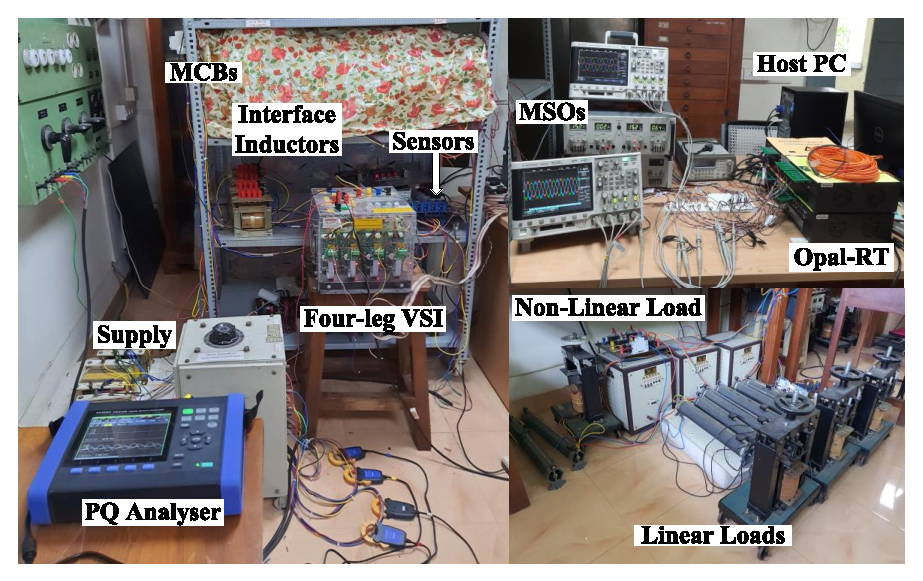
\includegraphics[scale=0.9]{figures/Chapter_5/Mine/Hardware_Picture_modified}
	\caption{Experimental prototype of the four-leg DVR}  
	\label{fig5.11}
\end{figure} 

In the experimental setup, the three-phase power supply is first stepped down to $50\,\si{V}$ per phase using a three-phase autotransformer. To introduce various voltage anomalies, a combination of a three-phase and a single-phase autotransformer pair is employed. The results obtained for a balanced voltage sag of $0.5\,\si{pu}$ on the grid voltage are presented in Fig.\,\ref{5.BalSag}. The figure displays the grid voltages ($v_{gabc}$), DVR injected voltages ($v_{Dabc}$), load voltages ($v_{labc}$), and load currents ($i_{labc}$). Note that the load currents are not shown for other voltage anomaly studies as they remain the same. 
During normal grid voltage conditions, it can be observed that the DVR injected voltages are almost zero. During the voltage sag period, the DVR injected voltages become non-zero to maintain the load voltages almost constant. This demonstrates the effectiveness of the proposed sliding mode control in mitigating voltage sags and maintaining load voltage quality. 
Furthermore, the total harmonic distortions (THDs) of the load voltages in phases $a$, $b$, and $c$ are evaluated during normal grid conditions and the balanced sag condition. For normal grid conditions, the THDs of load voltages in phases $a$, $b$, and $c$ are recorded as 2.58\%, 3.36\%, and 2.85\%, respectively. During the balanced sag condition, the THDs of load voltages in phases $a$, $b$, and $c$ are measured as 4.09\%, 5.45\%, and 4.11\%, respectively. These THD values provide an indication of the load voltage distortion levels and show the effectiveness of the DVR in reducing voltage harmonics and maintaining load voltage quality even during voltage sag events.
\begin{figure}[t!] %\vspace*{-0.5cm}  
	\centering
	\includegraphics[scale=1]{figures/Chapter_5/Mine/BalancedSag}
	\caption{Proposed SMC based four-leg DVR during balanced sag}  
	\label{5.BalSag}
\end{figure}

Fig.\,\ref{5.BalSwell} illustrates the behavior of the grid voltages ($v_{gabc}$), DVR injected voltages ($v_{Dabc}$), and load voltages ($v_{labc}$) during a balanced voltage swell event of $1.5\,\si{pu}$ on the grid voltage. It can be observed that under normal grid voltage conditions, the DVR injected voltages are close to zero, indicating minimal compensation required. However, during the voltage swell period, the DVR injected voltages become non-zero and are phase-opposed to the grid voltages. This counteraction helps to maintain stable load voltages by compensating for the excessive grid voltage rise.
Additionally, the THDs of the load voltages in phases $a$, $b$, and $c$ are evaluated during the balanced swell condition. The THDs of load voltages in phases $a$, $b$, and $c$ are recorded as 2.89\%, 3.34\%, and 2.22\%, respectively. The relatively low THD values demonstrate the effectiveness of the DVR in mitigating voltage swell impacts and maintaining the quality of load voltages.
\begin{figure}[t!] %\vspace*{-0.5cm}  
	\centering
	\includegraphics[scale=1]{figures/Chapter_5/Mine/BalancedSwell_No_IL}
	\caption{Proposed SMC based four-leg DVR during balanced swell}  
	\label{5.BalSwell}
\end{figure} 
\begin{figure}[t!]   
	\centering
	\includegraphics[scale=1]{figures/Chapter_5/Mine/UnbalancedSag1_No_IL} 
	\caption{Proposed SMC based four-leg DVR during single-phase unbalanced sag} %\vspace*{-0.5cm}
	\label{fig5.9}
\end{figure}

Fig.\,\ref{fig5.9} depicts the behavior of the grid voltages ($v_{gabc}$), DVR injected voltages ($v_{Dabc}$), and load voltages ($v_{labc}$) during an unbalanced voltage sag event specifically on phase-$b$ grid voltage (i.e., $V_{gb}=0.5\,\si{pu}$). From the figure, it is evident that the DVR injected voltages on phases-$a$ and $c$ remain close to zero throughout both normal grid voltage conditions and the unbalanced sag on grid voltages. This indicates that minimal compensation is required for phases-$a$ and $c$ as their grid voltages remain unaffected.
However, the DVR voltage on phase-$b$ is close to zero during normal grid voltage, but it becomes non-zero and compensates for the voltage sag on the respective phase grid voltage during the sag event. This active compensation helps in maintaining the load voltages at the desired levels, ensuring that they are not affected by the single-phase unbalanced grid voltage sag.
During the unbalanced sag in phase-$b$ grid voltage, the THDs of the load voltages in phases $a$, $b$, and $c$ are recorded as 2.25\%, 3.62\%, and 2.48\%, respectively. The relatively low THD values demonstrate the effectiveness of the DVR in mitigating voltage sag impacts and maintaining the quality of load voltages even in the presence of unbalanced grid conditions.

Fig.\,\ref{fig5.10} displays the grid voltages ($v_{gabc}$), DVR injected voltages ($v_{Dabc}$), and load voltages ($v_{labc}$) during an unbalanced voltage swell event occurring on phase-$a$ and phase-$c$ grid voltages (i.e., $V_{ga}=V_{gc}=1.5\,\si{pu}$).
From the figure, it can be observed that the DVR injected voltage on phase-$b$ remains relatively close to zero throughout both normal grid voltage conditions and the unbalanced swell on grid voltages. This indicates that minimal compensation is required for phase-$b$ as its grid voltage remains unaffected by the swell event.
On the other hand, the DVR voltages on phases-$a$ and $c$ are close to zero during normal grid voltage, but they become non-zero and actively compensate for the voltage swell on the respective phases. This active compensation ensures that the load terminal voltages are not impacted by the grid fluctuations and are maintained at the desired levels.
During the unbalanced two-phase swell condition, the THDs of the load voltages in phases $a$, $b$, and $c$ are recorded as 2.62\%, 2.59\%, and 1.81\%, respectively. The relatively low THD values demonstrate the effectiveness of the DVR in mitigating voltage swell impacts and preserving the quality of load voltages even in the presence of unbalanced grid conditions.
\begin{figure}[t!]   
	\centering
	\includegraphics[scale=1]{figures/Chapter_5/Mine/UnbalancedSwell2_No_IL}
	\caption{Proposed SMC based four-leg DVR during two-phase unbalanced swell} %\vspace*{-0.3cm}
	\label{fig5.10}
\end{figure} 
\begin{figure}[t!]   
	\centering
	\includegraphics[scale=1]{figures/Chapter_5/Mine/Various_modes}
	\caption{Proposed SMC based four-leg DVR during various modes of operations} %\vspace*{-0.3cm}
	\label{fig5.12}
\end{figure} 

Fig.\,\ref{fig5.12} illustrates the behavior of various system variables and signals during different system conditions. The following time instances correspond to specific events:
\begin{enumerate}
	\item At time $t_1$, the grid experiences an unbalanced sag on phase-$b$ grid voltage ($V_{gb}=0.5\,\si{pu}$). \vspace*{-0.5cm}
	\item At time $t_2$, the grid voltage recovers to normal mode. \vspace*{-0.5cm}
	\item At time $t_3$, the grid encounters an unbalanced swell on phase-$b$ grid voltage ($V_{gb}=1.5\,\si{pu}$). \vspace*{-0.5cm}
	\item At time $t_4$, the grid voltage returns to normal. \vspace*{-0.5cm}
	\item At time $t_5$, an additional load is connected to the grid. \vspace*{-0.5cm}
	\item At time $t_6$, the additional load is disconnected. \vspace*{-0.5cm}
	\item At time $t_7$, the reference neutral-point voltage ($v^{*}_{f^{\prime}o}$) is changed from $50\,\si{V}$ to $0\,\si{V}$. \vspace*{-1.3cm}
	\item At time $t_8$, the reference neutral-point voltage ($v^{*}_{f^{\prime}o}$) is set back to $50\,\si{V}$. \vspace*{-0.5cm}
\end{enumerate}
Examining Fig.\,\ref{fig5.12}, it can be observed that the DVR injected voltage on phase-$b$ remains close to zero during normal grid voltages, regardless of changes in load powers or the reference neutral-point voltage ($v^{*}_{f^{\prime}o}$). However, during periods of voltage sag or swell on the phase-$b$ grid voltage, the DVR voltage on phase-$b$ becomes non-zero to regulate the load voltage to the desired value.
The neutral-point voltage ($v_{f^{\prime}o}$) is a high-frequency pulsed waveform and is passed through a low-pass filter (LPF) with a cut-off frequency of $15\,\si{Hz}$. The filtered voltage, known as the averaged neutral-point voltage ($v_{f^{\prime}o\_flt}$), shown in Fig.\,\ref{fig5.12}, tracks its reference neutral-point voltage ($v^{*}_{f^{\prime}o}$).
The state variable $x_{b1}$ remains close to zero for various conditions, indicating that the actual voltage $v_{cb}$ accurately tracks its reference $v^{*}_{cb}$.
Based on the observations from Fig.\,\ref{fig5.12}, it can be concluded that the proposed algorithm effectively tracks both the DVR reference voltages and the reference neutral-point voltage, ensuring proper regulation and control of the system under different operating conditions.

\section{SUMMARY}
This chapter introduces the design of sliding mode control (SMC) in the natural reference frame for a four-leg dynamic voltage restorer (DVR) using a voltage source converter. The conventional approach of assigning appropriate values to the control inputs based on sliding variables faces challenges, which are addressed by the proposed sliding variables.
The proposed sliding variable for each leg of the converter is a combination of the respective filter-capacitor voltage and a fictitious voltage. The fictitious voltage is defined based on the converter's neutral-point voltage (NPV). This incorporation of the NPV control into the SMC scheme extends the control capabilities beyond just the compensation voltages of the DVR.
Furthermore, the chapter presents the selection of optimum sliding coefficients to maximize the sliding existence region for the four-leg DVR. This ensures robust and effective control performance.
To validate the performance of the DVR and the associated control scheme, detailed experimental studies are conducted under various operating conditions. The experimental results demonstrate the effectiveness of the proposed control approach in achieving accurate compensation performance.

Overall, the chapter provides insights into the design and implementation of SMC for a four-leg DVR, highlighting the importance of the proposed sliding variables and the optimization of sliding coefficients for enhanced control performance. The experimental validation further strengthens the credibility of the proposed approach.

